% gjilguid2e.tex
% V2.0 released 1998 December 18
% V2.1 released 2003 October 7 -- Gregor Hutton, updated the web address for the style files.

%\documentclass[extra,mreferee]{gji}
\documentclass[extra]{gji}

\bibliographystyle{gji}
\usepackage{timet}
\usepackage[dvips]{graphicx}

\title{Relocating a cluster of earthquakes using a single station}
\author[D.J. Robinson, M. Sambridge, R. Snieder and J Hauser]
  {David J. Robinson$^{1,2}$, Malcolm Sambridge$^{1}$, Roel Snieder$^{3}$, J\"urg Hauser$^{4}$ \\
  $^1$ Research School of Earth Sciences, Australian National
    University, Canberra ACT \emph{0200}, Australia, E-mail: david.robinson@anu.edu.au \\
$^2$  Risk Research Group, Geoscience Australia, GPO Box \emph{383} Canberra ACT \emph{2601} Australia, E-mail: david.robinson@ga.gov.au\\
$^3$ Center for Wave Phenomena and Department of Geophysics, Colorado School of Mines, Golden CO \emph{80401-1887}, USA \\
$^4$ Earthquakes and the Environment Program, NORSAR,Kjeller, Norway}




\date{Received 2010 Month Day; in original form 2010 Month Day}
\pagerange{\pageref{firstpage}--\pageref{lastpage}}
\volume{200}
\pubyear{2010}

%\def\LaTeX{L\kern-.36em\raise.3ex\hbox{{\small A}}\kern-.15em
%    T\kern-.1667em\lower.7ex\hbox{E}\kern-.125emX}
%\def\LATeX{L\kern-.36em\raise.3ex\hbox{{\Large A}}\kern-.15em
%    T\kern-.1667em\lower.7ex\hbox{E}\kern-.125emX}
% Authors with AMS fonts and mssymb.tex can comment out the following
% line to get the correct symbol for Geophysical Journal International.
\let\leqslant=\leq

\newtheorem{theorem}{Theorem}[section]

\begin{document}

\label{firstpage}

\maketitle


\begin{summary}
(Type abstract here)
\end{summary}

\begin{keywords}
 Probability distributions; Earthquake source observations; Seismicity and tectonics; Wave scattering and diffraction
\end{keywords}

\section{Introduction}

Earthquake location is important for many applications. It assists
our understanding of seismic activity by indicating regions of
relatively higher seismicity such as major lithospheric plate
boundaries \citep[e.g., ][]{dr_Sykes67a, dr_Isacks68a,
dr_Stein02a} or local active source zones
\citep[e.g., ][]{dr_Gutenberg44a, dr_Giardini03a}.
Earthquake locations are required for  magnitude determination
\citep[e.g., ][]{dr_Richter35a, dr_Gutenberg45a}, computing
moment tensors \citep[e.g., ][]{dr_Sipkin02a} and
seismological studies of the Earth's interior
\citep[e.g., ][]{dr_Spencer80a, dr_Kennett95a, dr_Curtis02a,
dr_Kennett04a}. They are needed to
understand strong motion and seismic attenuation
\citep[e.g., ][]{dr_Toro97a, dr_Campbell03a}
 and model earthquake hazard or risk
\citep[e.g., ][]{dr_Frankel00a, dr_Stirling02a, dr_Robinson06b}.
The accuracy required in earthquake location depends on the application.
For example, imaging the structure of a fracture system from microseismicity
requires greater detail than determining whether a $M_w=7.5$ earthquake
occurs offshore for tsunami warning purposes. This paper focuses
on reducing the uncertainty on the locations of a cluster of events, particularly
when they are recorded by a small number of stations.

Absolute location describes the location of an earthquake
with respect to some global reference such as latitude, longitude (or
easting/northing) and depth. Uncertainties associated with absolute locations
are influenced by source to station distances, the number of
stations and their geometry, quality of signal and accuracy of
the velocity model used in computing travel times. Errors in absolute location are typically of the
order of several km because they are susceptible to uncertainty in the velocity
structure along the entire path between the source and receiver.
For example, \citet{dr_Shearer99a} states that location uncertainty
in the ISC and PDE catalogues are generally around 25\,km horizontally and
at least 25\,km in depth.\footnote{Here the depth uncertainties of 25\,km assume the use
of depth dependent phases such as $pP$. Without such phases the uncertainty is higher.}
  These locations are created using global seismic networks.
\citet{dr_Bondar04a} demonstrate
that at the local scale, absolute locations are accurate to within 5\,km with a 95\%
confidence level when local networks meet a number of station
related criteria. Such errors are too large for many applications, particularly
those focussed on the study of micro seismicity and imaging
rupture surfaces from aftershock sequences.

Relative earthquake location involves locating a group of earthquakes with
respect to one another and was first introduced by \citet{dr_Douglas67a}
who developed the technique commonly known as joint hypocenter
determination.\footnote{\citet{dr_Douglas67a} originally used the term
joint epicentre determination. However, he was solving for hypocentre.}
In principle, relative locations can be
computed by differencing absolute locations. However, \citet{dr_Pavlis92a}
shows that inadequate knowledge of velocity structure leads to
systematic biases when relative positions are computed in this way.
This is confirmed by \citet{dr_Richards06a}
who state that inaccuracies in the travel time model are one of
two primary error sources in absolute earthquake location. The other
error source is erroneous arrival picks. To reduce errors from the travel
time model, relative location techniques compute locations
directly from travel time differences between two waveforms
\citep[e.g., ][]{dr_Ito85a, dr_Got94a, dr_Nadeau97a, dr_Waldhauser99a}.
By doing so, they remove errors
associated with unknown lateral velocity variations outside the
local region, because such variations influence all waveforms in
the same manner \citep{dr_Shearer99a}.

Reported uncertainties
for event locations from relative techniques are  around 15 to 75\,m in
local settings with good station coverage
\citep[e.g., ][]{dr_Ito85a, dr_Got94a, dr_Waldhauser99a,dr_Waldhauser08a}.
Here, `good coverage' implies multiple
stations distributed across a broad range of azimuthal directions.
Precise relative location techniques have been applied to a
diverse range of problems. For example, the location of active
fault planes \citep[e.g., ][]{dr_Deichmann92a, dr_Got94a,
dr_Waldhauser99a, dr_Waldhauser02a, dr_Shearer05a}, studying rupture mechanics
\citep[e.g., ][]{dr_Rubin99a, dr_Rubin02a}, interpreting magma
movement in volcanoes \citep[e.g., ][]{dr_Fremont87a} and monitoring
pumping induced seismicity \citep[e.g., ][]{dr_Lees98a,
dr_Ake05a}. \citet{dr_Poupinet84a},
\citet{dr_Bokelmann00a} and  \citet{dr_Rubin02b} apply relative
location techniques to identify earthquake doublets, events that have near identical
locations. \citet{dr_Poupinet84a} use these doublets to measure
temporal variation in crustal velocity, \citet{dr_Bokelmann00a}
use them to identify systematic temporal variations in seismic
anisotropy and \citet{dr_Rubin02b} describes how they are useful for
correcting time-dependent station delays.

In traditional approaches to absolute and relative location
only early onset body waves, typically $P$ and/or $S$ waves, are used.
The data utilised may be the direct arrival times; the travel time difference computed
between direct arrivals of two waveforms; or the time differences
inferred from time-lagged cross correlation of relatively small windows
around the body wave arrivals.
 In all three cases, the majority of the
waveform is discarded. Furthermore, obtaining high accuracy with these techniques
requires multiple stations with good azimuthal coverage.
In this paper we demonstrate that it is possible to
significantly reduce location uncertainty when few stations are
available by using more of the waveform.

Coda refers to  later arriving waves in the seismogram that arise from
scattering  \citep{dr_Aki69a,dr_Snieder99a,dr_Snieder06a}.
Typically, the coda waves are ignored in most seismological
applications due to the complexity involved in modeling their
generation. In this
paper we develop an approach for locating earthquakes using coda waves.
\citet{dr_Snieder05a} demonstrate that the
coda of two earthquakes can be used to estimate the separation between
them. Their technique is based on the interference pattern between
the coda waves and is known as coda wave interferometry (CWI).
Unlike travel time techniques, CWI
 does not require multiple stations or good azimuthal coverage.
In fact, it is possible to obtain estimates of separation using a single
station \citep{dr_Robinson07b}. This makes CWI particularly interesting
for regions where station density is low such as intraplate areas.
Our technique can be used on coda waves alone or in combination with
travel times. We demonstrate that the use of coda waves improves
the location of a cluster of events when the recording situation
is poor and we show that it is possible to obtain accurate relative locations with as
little as one station.

\section{Theory}

\citet{dr_Snieder05a} introduce a CWI based estimator of source
separation $\delta_{CWI}$ between two earthquakes
\begin{equation}
\label{eq:Theory-dcwi_g_sigmat}
\delta_{CWI}^2 = g(\alpha,\beta)\sigma_\tau^2,
\end{equation}
where $\sigma_\tau$ is the standard deviation of the travel time perturbation
between the coda waves of two earthquakes,
and $\alpha$ and $\beta$ are the near source $P$ and $S$ wave velocities,
respectively. The function $g$ depends on the type of excitation
(explosion, point force, double couple) and on the direction of
source displacement relative to the point force or double
couple. For example, for two double couple sources displaced in the
fault plane,
\begin{equation}
\label{eq:LitReview-g-3d-dc}
g(\alpha,\beta) = 7
\frac{\left(\frac{2}{\alpha^6}+\frac{3}{\beta^6}\right)}{\left(\frac{6}{\alpha^8}+\frac{7}{\beta^8}\right)},
\end{equation}
whereas, for two point sources in a 2D acoustic medium
\begin{equation}
\label{eq:LitReview-g-2d-ps} g(\alpha,\beta) = 2 \alpha^2
\end{equation}
\citep{dr_Snieder05a}. The
$\sigma_\tau$ in eq. (\ref{eq:Theory-dcwi_g_sigmat}) is related to $R_{max}$, the maximum of the cross correlation between
the coda of the two waveforms and hence can be computed directly from the recorded data.
In this paper we use the autocorrelation
approach of \citet{dr_Robinson10b} when relating these parameters
and we apply a restricted time lag search when evaluating $R_{max}$. These extensions
to the original technique of \citet{dr_Snieder05a} increase the range of applicability
of CWI by 50\%.

\citet{dr_Robinson10b} show that coda waves provide
only probabilistic constraints on source separation and
introduce a Bayesian approach for describing the probability
of true separation given the CWI data. Their approach is
summarised by
\begin{equation}
\label{eq:-bayesian-noisyform}
P(\widetilde{\delta}_t|\widetilde{\delta}_{CWIN}) \propto P(\widetilde{\delta}_{CWIN}|\widetilde{\delta}_t)
\times P(\widetilde{\delta}_t)
\end{equation}
where  $P(\widetilde{\delta}_t|\widetilde{\delta}_{CWIN})$ is the posterior function
indicating the probability of true separation $\widetilde{\delta}_t$ given the noisy CWI separation
estimates $\widetilde{\delta}_{CWIN}$; $P(\widetilde{\delta}_{CWIN}|\widetilde{\delta}_t)$
is the likelihood function representing the forward model between the
desired separation $\widetilde{\delta}_t$ and the data $\widetilde{\delta}_{CWIN}$; and
$P(\widetilde{\delta}_t)$ is the prior function accounting for all a-priori information.
The tilde above the separation parameters in eq. (\ref{eq:-bayesian-noisyform})
indicates the use of a wavelength normalised separation parameter
\begin{equation}
\label{eq-normalisation-eqn}
\widetilde{\delta} = \frac{\delta}{\lambda_{d}},
\end{equation}
which measures separation ($\delta$ = $\delta_{CWIN}$ or $\delta_t$) with
respect to dominant wavelength $\lambda_{d}$.
In this paper we consider a uniform prior which gives emphasis to the recorded data.
The algorithm for computing the noisy
likelihood $P(\widetilde{\delta}_{CWIN}|\widetilde{\delta}_t)$ is derived by \citet{dr_Robinson10b}
and summarised in Appendix \ref{sec-Appendix-noisylikelihood}. With these two pieces
in place we can compute the posterior $P(\widetilde{\delta}_t|\widetilde{\delta}_{CWIN})$
(or PDF) for the separation between any pair of events directly from their coda waves.

We seek a probability density function (PDF) which links
 individual pairwise posteriors $P(\widetilde{\delta}_t|\widetilde{\delta}_{CWIN})$
and describes the location of multiple events with maximum identifying
 the most probable combination of locations.
More importantly however, the PDF will
quantify location uncertainty and provide information
on the degree to which individual events are constrained
 by the data. For convenience, we begin with three earthquakes having locations
$\mathbf{e}_1$, $\mathbf{e}_2$ and $\mathbf{e}_3$. Using a Bayesian formulation we write
\begin{equation}
\label{eq-Bayes-three-locations}
P(\mathbf{e}_1, \mathbf{e}_2, \mathbf{e}_3| \mathbf{d}) \propto P( \mathbf{d}|\mathbf{e}_1, \mathbf{e}_2, \mathbf{e}_3)
\times P(\mathbf{e}_1, \mathbf{e}_2, \mathbf{e}_3),
\end{equation}
where $P(\mathbf{e}_1, \mathbf{e}_2, \mathbf{e}_3 | \mathbf{d})$, $P(\mathbf{d}|\mathbf{e}_1, \mathbf{e}_2, \mathbf{e}_3)$
and $P(\mathbf{e}_1, \mathbf{e}_2, \mathbf{e}_3)$ are the posterior,
likelihood and prior functions, respectively. In eq. (\ref{eq-Bayes-three-locations})
$\mathbf{d}$ represents observations that constrain the locations. They can be any combination
of travel times, geodetic information  or CWI separation estimations. For example, if coda waves are used
we have $P(\mathbf{e}_1, \mathbf{e}_2, \mathbf{e}_3 | \widetilde{\mitbf{\delta}}_{CWIN})$ and
$P(\widetilde{\mitbf{\delta}}_{CWIN}|\mathbf{e}_1, \mathbf{e}_2, \mathbf{e}_3)$
where $\widetilde{\mitbf{\delta}}_{CWIN}$ are the wavelength normalised separation estimates.
Alternatively, if we use CWI and travel time data we may write
$P(\mathbf{e}_1, \mathbf{e}_2, \mathbf{e}_3 | \widetilde{\mitbf{\delta}}_{CWIN}, \mathbf{t}_{DD})$ and
$P(\widetilde{\mitbf{\delta}}_{CWIN},\mathbf{t}_{DD}|\mathbf{e}_1, \mathbf{e}_2, \mathbf{e}_3)$
where $\mathbf{t}_{DD}$ represent travel time differences.
In this derivation and in Sec. \ref{sec:benchmarking} we focus on the constraints imposed by coda waves, whereas in
Sec. \ref{sec:CalaverasLoc-CWIandTT} we demonstrate how
CWI and travel time data can be combined.

For three earthquakes we have likelihoods;
$P(\widetilde{\delta}_{CWIN,12}|\mathbf{e}_1, \mathbf{e}_2)$,
$P(\widetilde{\delta}_{CWIN,13}|\mathbf{e}_1, \mathbf{e}_3)$
and
$P(\widetilde{\delta}_{CWIN,23}|\mathbf{e}_2, \mathbf{e}_3)$.
In writing
these likelihoods we have replaced the conditional term on separation
$\widetilde{\delta}_t$ with the locations (e.g. $\mathbf{e}_1$ and $\mathbf{e}_2$).
This can be done because
knowledge of location translates to separation.\footnote{Note that the reverse
can not be said. That is, knowledge of separation between a single event pair
does not translate to location but rather places a non-unique constraint on
location.}
Furthermore, since the pairwise functions are independent the joint
likelihood becomes
\begin{equation}
\begin{array}{l}
\label{eq:-joint-likelihood4three}
P(\widetilde{\mathbf{\delta}}_{CWIN} | \mathbf{e}_1, \mathbf{e}_2, \mathbf{e}_3) =
P(\widetilde{\delta}_{CWIN,12} | \mathbf{e}_1, \mathbf{e}_2) \\
\hspace{2em} \times P(\widetilde{\delta}_{CWIN,13} | \mathbf{e}_1, \mathbf{e}_3)
\times  P(\widetilde{\delta}_{CWIN,23} | \mathbf{e}_2, \mathbf{e}_3).
\end{array}
\end{equation}
Similarly, we note that earthquake locations are independent and the
joint prior becomes
\begin{equation}
\label{eq:-joint-prior4three}
P(\mathbf{e}_1, \mathbf{e}_2, \mathbf{e}_3) = P((\mathbf{e}_1) \times P(\mathbf{e}_2) \times P(\mathbf{e}_3).
\end{equation}
Combining eqs. (\ref{eq:-joint-likelihood4three}) and (\ref{eq:-joint-prior4three})
gives the joint posterior function
\begin{equation}
\label{eq-3eqposterior}
\begin{array}{l}
P(\mathbf{e}_1, \mathbf{e}_2, \mathbf{e}_3 | \widetilde{\mitbf{\delta}}_{CWIN}) = c \displaystyle \prod_{i=1}^3 P(\mathbf{e}_i) \\
\hspace{4em}  \times \displaystyle \prod_{i=1}^2 \prod_{j=i+1}^3 P(\widetilde{\delta}_{CWIN,ij}|\mathbf{e}_i,\mathbf{e}_j)
\end{array}
\end{equation}
for three events. A detailed understanding of the location of a single event (e.g. $\mathbf{e}_2$) is obtained by computing the
marginal
\begin{equation}
\label{eq:-E2-marginal}
P(\mathbf{e}_2) = \int \int P(\mathbf{e}_1, \mathbf{e}_2, \mathbf{e}_3 | \widetilde{\mathbf{\delta}}_{CWIN}) d\mathbf{e}_1 d\mathbf{e}_3
\end{equation}
where the intergral is taken over all plausible locations for $\mathbf{e}_1$ and $\mathbf{e}_3$.
Alternatively, we can compute the marginal for a single event coordinate
by integrating the posterior over all events and remaining coordinates
for the chosen earthquake. Evaluation of $c$ in eq. (\ref{eq-3eqposterior}) involves finding the value which
normalises the posterior function to unit area over all plausible locations.
In many applications the constant of
proportionality $c$ is not important. For example, it is not required
when seeking the combination of locations which maximise
 the posterior function, nor in Bayesian sampling algorithms such as Markov-chain Monte-Carlo
techniques which require evaluation of a function proportional to the PDF.

By following the same argument we get the posterior function
\begin{equation}
\begin{array}{l}
\label{posterior-n-events}
P(\mathbf{e}_1,...,\mathbf{e}_n | \widetilde{\mathbf{\delta}}_{CWIN}) = c \displaystyle \prod_{i=1}^n P(\mathbf{e}_i) \\
\hspace{4em} \displaystyle  \times \prod_{i=1}^{n-1} \prod_{j=i+1}^n P(\widetilde{\delta}_{CWIN,ij}|\mathbf{e}_i,\mathbf{e}_j)
\end{array}
\end{equation}
for $n$ events. When evaluating eq. (\ref{posterior-n-events}) over a range of locations
it is necessary to compute and multiply many numbers close to zero.
This is because the PDFs tend to zero as
the locations get less likely (i.e. near the boundaries of the plausible region).
Such calculations are prone to truncation errors so we
work with the negative logarithm
\begin{equation}
\label{eq:-negative-log-part1}
L(\mathbf{e}_1, \mathbf{e}_2, ..., \mathbf{e}_n) = -ln\left[ P(\mathbf{e}_1,...,\mathbf{e}_n | \widetilde{\mathbf{\delta}}_{CWIN} )  \right]
\end{equation}
or
\begin{equation}
\begin{array}{l}
\label{eq:-negative-log}
L(\mathbf{e}_1, \mathbf{e}_2, ..., \mathbf{e}_n) =
-ln\left[ c \right] - \displaystyle \sum_{i=1}^n ln\left[P(\mathbf{e}_i)\right] \\
\hspace{3em} - \displaystyle \sum_{i=1}^{n-1} \sum_{j=i+1}^n ln\left[P(\widetilde{\delta}_{CWIN,ij}|\mathbf{e}_i,\mathbf{e}_j)\right].
\end{array}
\end{equation}
The logarithm improves numerical stability by replacing products with summations. The negative assists with
optimisation, many algorithms for which are designed to minimise an objective function.

The event locations $\mathbf{e}_1, \mathbf{e}_2, ..., \mathbf{e}_n$
are defined by coordinates $\hat{x}$, $\hat{y}$ and $\hat{z}$
where the hat $\hat{.}$ indicates use of
a local coordinate system. We choose a local coordinate system
which removes ambiguity associated with transformations of the coordinate system,
such as translations and rotations, that do not change the distance between events.
In defining this coordinate system we fix the first event at the origin,
\begin{equation}
\label{eq:coord-const1}
\mathbf{e}_1 = (0,0,0),
\end{equation}
the second event on the positive $\hat{x}$-axis
\begin{equation}
\label{eq:coord-const2}
\mathbf{e}_2 = (\hat{x}_2, 0, 0), \hat{x}_2>0
\end{equation}
the third on the $\hat{x}-\hat{y}$ plane
\begin{equation}
\label{eq:coord-const3}
\mathbf{e}_3 = (\hat{x}_3,\hat{y}_3,0), \hat{y}_3>0
\end{equation}
and the fourth to
\begin{equation}
\label{eq:coord-const4}
\mathbf{e}_4 = (\hat{x}_4,\hat{y}_4,\hat{z}_4), \hat{z}_4>0.
\end{equation}
This coordinate system reduces translational (constraint \ref{eq:coord-const1})
and rotational (constraints \ref{eq:coord-const2} to \ref{eq:coord-const4}) non-uniqueness
without loss of generality. It is necessary to work with a local coordinate
system when using coda waves alone because the CWI technique constrains only event separation
between earthquakes. The inclusion of travel times in Sec. \ref{sec:CalaverasLoc-CWIandTT}
allows us to move to a global reference system.

In summary, the posterior $P(\mathbf{e}_1,...,\mathbf{e}_n | \widetilde{\mathbf{\delta}}_{CWIN})$ and its negative
logarithm $L$ describe the joint probability of multiple event locations given the observed coda waves.
The most likely set of locations is given by the minimum of $L$.   In this paper we use the Polak-Ribiere
technique \citep{dr_Press87a} to optimise $L$. The Polak-Ribiere
technique is a particular choice of conjugate gradient method. It uses the
derivatives of $L$ to guide the optimisation procedure. We derive the derivatives in Appendix \ref{sec-Appendix-derivatives_ofL}.

\subsection{Synthetic experiments}
\label{sec:benchmarking}

We use synthetic examples in 2D with 50 earthquakes to test the performance of the optimisation
routine.

\subsection{2D synthetic experiments}

Actual locations are created by
randomly selecting $\hat{x}$- and $\hat{y}$-coordinates such that $-50 \leq \hat{x} \leq 50$ and $-50 \leq \hat{y} \leq 50$.
These are indicated with triangles in Fig. \ref{fig-2D50eq-relocation_eg1}.
 We assume a local velocity of $v=3300\,$ms$^{-1}$ between all
event pairs and a dominant frequency of 2.5$\,$Hz to represent waveform data filtered between 1 and 5$\,$Hz.
The CWI data are defined by the positive bounded Gaussian with statistics
$\bar{\mu}_N$ and $\bar{\sigma}_N$. A hypothetical CWI mean is created by setting
\begin{equation}
\label{eq:hypothetical-CWI-mean-optichapt}
\bar{\mu}_N = \mu_1 \left( \widetilde{\delta}_t \right)
\end{equation}
using eq. (\ref{eq:mu1}). This assumption ensures that
the sample mean of hypothetical separation estimates is consistent with known CWI
biases \citep{dr_Robinson10b}. In example 1 we use $\bar{\sigma}_N=0.02$ between all event pairs.
Application of our optimisation procedure on the hypothetical CWI data yields the circles
in Fig. \ref{fig-2D50eq-relocation_eg1}. The optimisation does not lead to the correct
solution due to the addition of noise $\bar{\sigma}_N=0.02$ on the hypothetical
CWI data. The average coordinate error
is 2.0\,m which is small compared to the noise of $\bar{\sigma}_N=0.02$ which for
$v_s=3300$\,ms$^{-1}$ and $f_{dom}=2.5$\,Hz corresponds to roughly 25\,m.
\begin{figure}
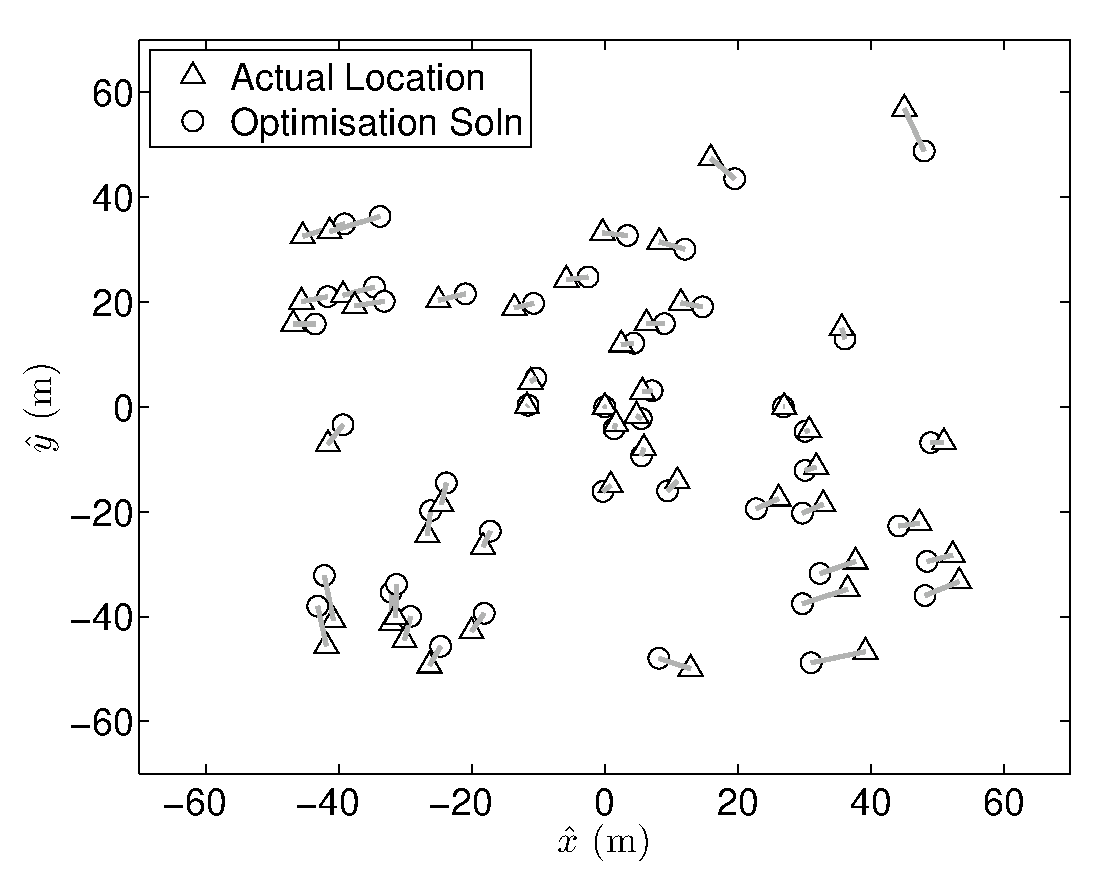
\includegraphics[width = 20pc]{diags/locs_2D_50eq_1.eps}
\caption{Example 1 - Synthetic relocation of 50 earthquakes in 2D using all constraints with noise $\bar{\sigma}_N=0.02$.
Actual and optimisation event locations
are shown in blue and red circles, respectively.}
\label{fig-2D50eq-relocation_eg1}
\end{figure}

\begin{figure}
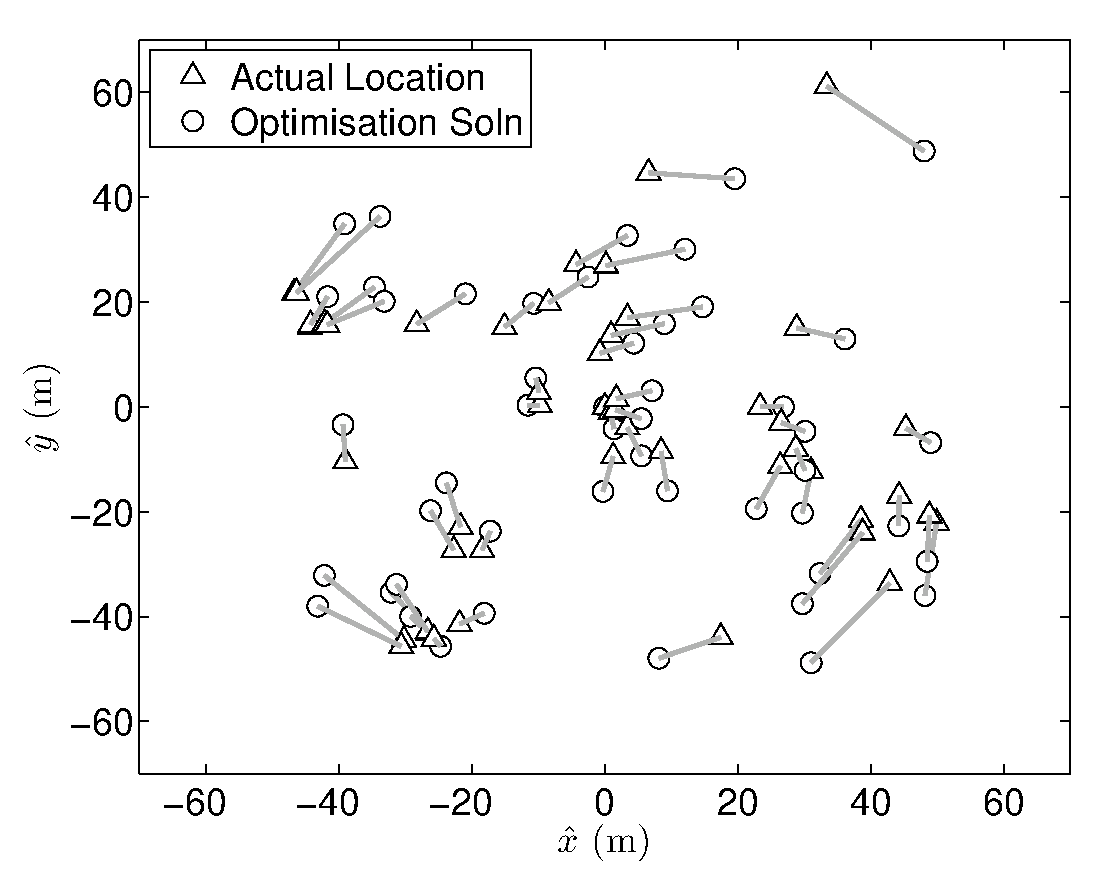
\includegraphics[width = 20pc]{diags/locs_2D_50eq_3.eps}
\caption{Example 3 - Synthetic relocation of 50 earthquakes in 2D using all constraints with noise
$\bar{\sigma}_N= 2 \sigma_{1to5Hz}(\delta_t)$.
 Actual and optimisation event locations
are shown in blue and red circles, respectively.}
\label{fig-2D50eq-relocation_eg3}
\end{figure}
\citet{dr_Robinson10b} demonstrates that the noise on CWI estimates is often larger than 0.02 and that it increases
with event separation. Consequently, example 1 is overly simplistic because we fix
$\bar{\sigma}_N=0.02$ for all pairs. In example 2 we increase the uncertainty and introduce a distance
dependance into the hypothetical $\bar{\sigma}_N$ by defining
$\bar{\sigma}_N=\sigma_{1to5Hz}(\delta_t)$, where $\sigma_{1to5Hz}(\delta_t)$ is the half-width of
the errorbars for a synthetic acoustic experiment
with filtering between 1 and 5\,Hz \citep[see Fig4(b) of ][]{dr_Robinson10b}.
Repeating the optimisation leads
to the circles in Fig. \ref{fig-2D50eq-relocation_eg3} which have an average coordinate error of 2.8\,m.

Conjugate gradient based optimisation techniques are susceptible to the presence of local minima.
This is because they use the slope of the target function to explore the solution space.
We explore the impact of local minima for our CWI location problem by beginning
the optimisation from 25 different randomly chosen starting positions. In this case we observe no differences
in the solution for neither examples 1 or 2.

We can draw three observations from the error structure in Figs. \ref{fig-2D50eq-relocation_eg1} and
\ref{fig-2D50eq-relocation_eg3}. Firstly, we note that the location errors depicted
by grey bars in each figure increase between examples 1 and 2 with the
introduction of larger noise. Secondly, the errors are larger for
events at greater distances from the center. This is because events near the center of the cluster are
constrained by links from all angles, whereas those
on the outside are moderated by links from a limited number of directions. This observation is analogous
to problems associated with poor azimuthal coverage in common triangulation problems such as individual earthquake location
from limited travel time data, or GPS positioning with few satellites. Our third observation is that the location errors appear to
be circular, despite our attempt to correct for rotational non-uniqueness with the local coordinate system.

The local coordinate system works by constraining the location of the first three
earthquakes. Earthquake 1 is fixed at the origin, earthquake 2 on the positive $\hat{x}$-axis and earthquake 3
has $\hat{y}>0$. As the number of events increases the strength of this constraint on later events
becomes weaker allowing small rotations of events with respect to each other.
That is, even though the rotational freedom of the cluster is in principal
removed by the constraints imposed on the events (see eqs. \ref{eq:coord-const1} to \ref {eq:coord-const4}) we observe that
in practice the effects of noise means that the rotational non-uniqueness
reappears. This is because the `easiest' way data noise can propagate is into
the direction which is least constrained by the data. It is the same phenomena as in
linear inversion where noise creates large spurious model changes in directions
of the eigenvectors with the smallest singular values \citep[e.g ][]{dr_Aster05a}.
Unfortunately, there is no obvious way to overcome this issue when using coda
waves alone since the constraints are based on separation. Fortunately however, combining coda waves with
measurements of travel times alleviates this problem and facilitate the removal of a local coordinate system
altogether.

Despite these observations about the error structure however, we gain confidence in the
optimisation procedure due to its stability for different starting locations and
because of the small average coordinate errors of 2.0\,m and 2.8\,m
for examples 1 and 2, respectively.

\subsubsection{The impact of reduced linkage}

A set of earthquakes and their corresponding coda wave estimates of separation can be thought of as
a network. In this network the earthquakes are nodes and the constraints are branches or links
which join them together. Synthetic examples 1 and 2 use 100\% direct linkage between event pairs. That is, there is a constraint
between each earthquake and all other events. In reality, we might expect that the separation between some
pairs will not be constrained by CWI data due to poor signal to noise ratio in the coda for common stations.
Obviously, the less stations that record an event the more likely it is that links
between it and other events will be broken.
In such cases the probabilistic distance constraint between a pair of
events may only exist indirectly through multiple pairs. In this section we
consider the impact of reduced linkage between event pairs. In example 3, we repeat example 2
using 90\%, 80\%, ..., 10\% of the links. As with the above examples, we undertake the
optimisation with 25 randomly chosen starting locations.

\begin{figure}
%\noindent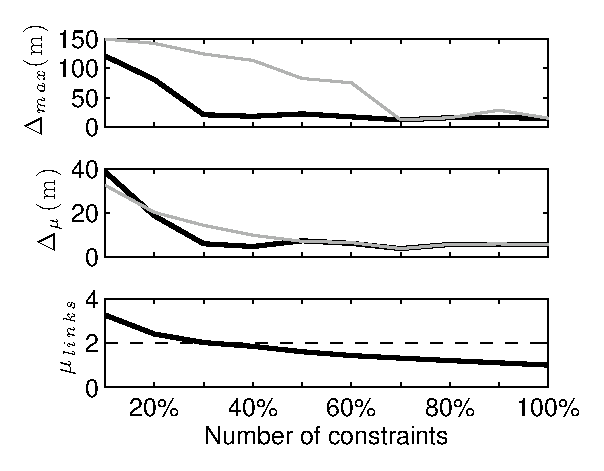
\includegraphics[width = 20pc]{../../thesis_version2/diags/eq_location_optimisation/synth2Dmulti/ressummary_2Dsynth50eq.eps}
\noindent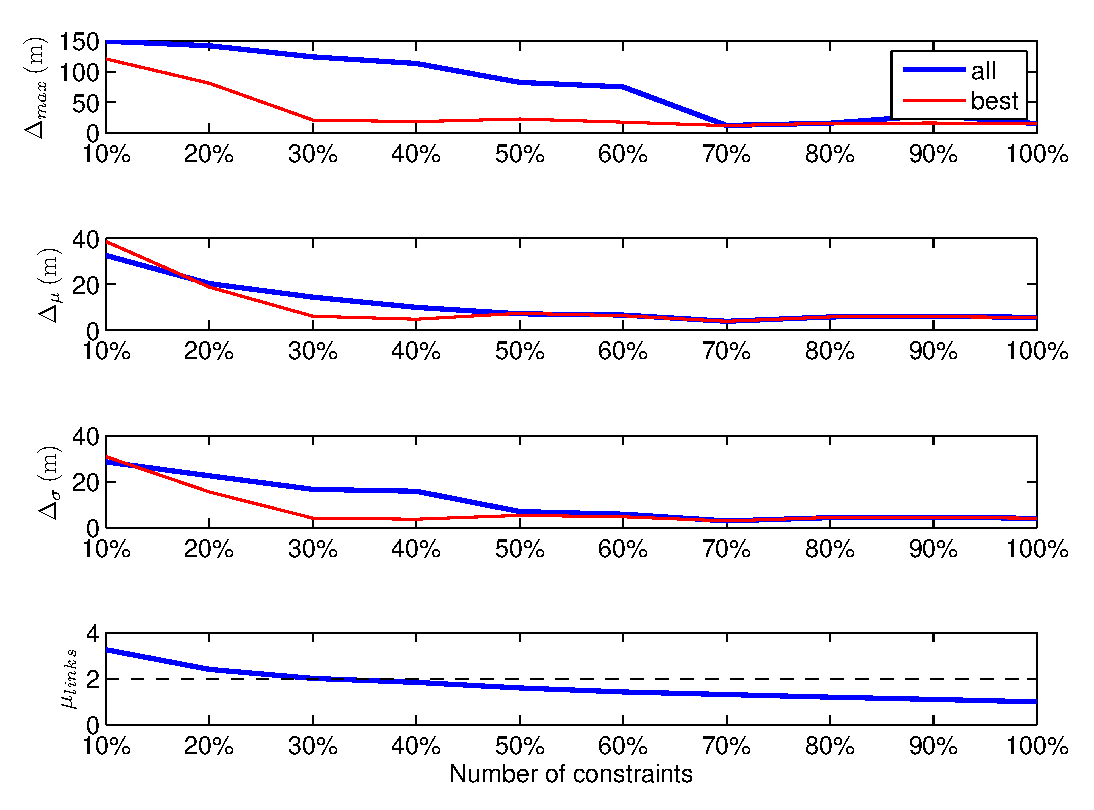
\includegraphics[width = 20pc]{diags/ressummary_2Dsynth50eq.eps}
\caption{Statistical measures of error in the optimisation solutions for the 2D synthetic cases when all (blue)
and best (red) results are considered. The statistics $\Delta_{max}$, $\Delta_\mu$ and
$\Delta_\sigma$ are the maximum, mean and standard deviation of the coordinate error, respectively.
The bottom subplot shows the average minimum number of branches required to link the 2450 pairs.}
 \label{fig:optimisationresults-2Dsynth}
\end{figure}

In Figs. \ref{fig:optimisationresults-2Dsynth}(a) and (b) we examine the performance of the optimisation statistically. In particular,
we plot the maximum $\Delta_{max}$ and mean $\Delta_\mu$ of the coordinate difference as a function of increasing linkage.
We show the statistics for the `best' optimisation solution (black) and for the solution space
when all 25 optimisations are considered (grey). In this case the best solution is determined
by the set of event locations which lead to the smallest value of $L$.
We observe similar errors in the best solution for all cases when at least 30\% of the
branches are used. The errors increase drastically when only 10\% or 20\% of the constraints are included.
Interestingly, this breakdown around 20\% to 30\% coincides with the point where the average number of branches
required to link each pair reaches 2 (see Fig.\ref{fig:optimisationresults-2Dsynth}(c)). Since the average number of branches can be computed
in advance it can be used as an indication of the potential stability of the inversion prior
to optimisation. An earlier breakdown is observed when all 25 solutions
are considered collectively. For example, the
maximum coordinate error $\Delta_{max}$ is significantly higher than that for the best solution for all
cases with 60\% of the constraints or less. This observation suggests that
the optimisation is susceptible to the presence of local minima and that a range of starting points
should be considered.

Interestingly, we note that some of the optimisations chains
fail to converge after 1200 iterations when the linkage is 60\% or lower and all
fail when then linkage is 20\% or lower. Despite their failure to converge however, many of the
solutions remain relatively close to the actual solutions. The derivatives used in the conjugate gradient method
depend on events connected by CWI measurements. Consequently,
earthquakes that are only connected via other events do not `communicate' with each other
directly. To some extent, this should be taken care of during the iterative process where location information
can spread to events which have no direct links. However, the
lack of connection through the gradient could prevent convergence in extreme cases, or more likely
slow the procedure down. This could explain why some
examples do not converge after 1200 iterations.
\citet{dr_VanDecar94a} show that gradient damping acts
slowly through iterative least-squares, because
 every cell in one iteration communicates only with its neighbours, and they demonstrate that this can be
fixed with preconditioning in some cases. Their findings suggest that it may be possible to improve
the convergence (stability and/or speed) of the CWI optimisation by preconditioning.

\subsubsection{3D synthetic examples with reduced linkage}

In this section we expand the optimisation routine to 3D and repeat example 3 of the 2D case.
We randomly pick a set of actual event locations for 50 earthquakes with
$-50$\,m$\leq \hat{x},\hat{y},\hat{z} \leq 50$\,m. As in the 2D case we assume a local velocity
of $v=3300\,$ms$^{-1}$ between all event pairs and a dominant frequency of 2.5$\,$Hz to represent
 waveform data filtered between 1 and 5$\,$Hz.
The hypothetical CWI mean is created using eq. \ref{eq:hypothetical-CWI-mean-optichapt}
which ensures consistency between the sample mean of hypothetical separation estimates and CWI
biases. We use a standard deviation for the noisy CWI estimates
of $\bar{\sigma}_N = \sigma_{1to5Hz}$ and perform the optimisation using 10\%,
20\%, ..., 100\% of the direct links.
In each case we repeat the
optimisation 25 times using randomly chosen starting locations. The results are
summarised in Fig. \ref{fig:optimisationresults-3Dsynth}.

\begin{figure}
%\noindent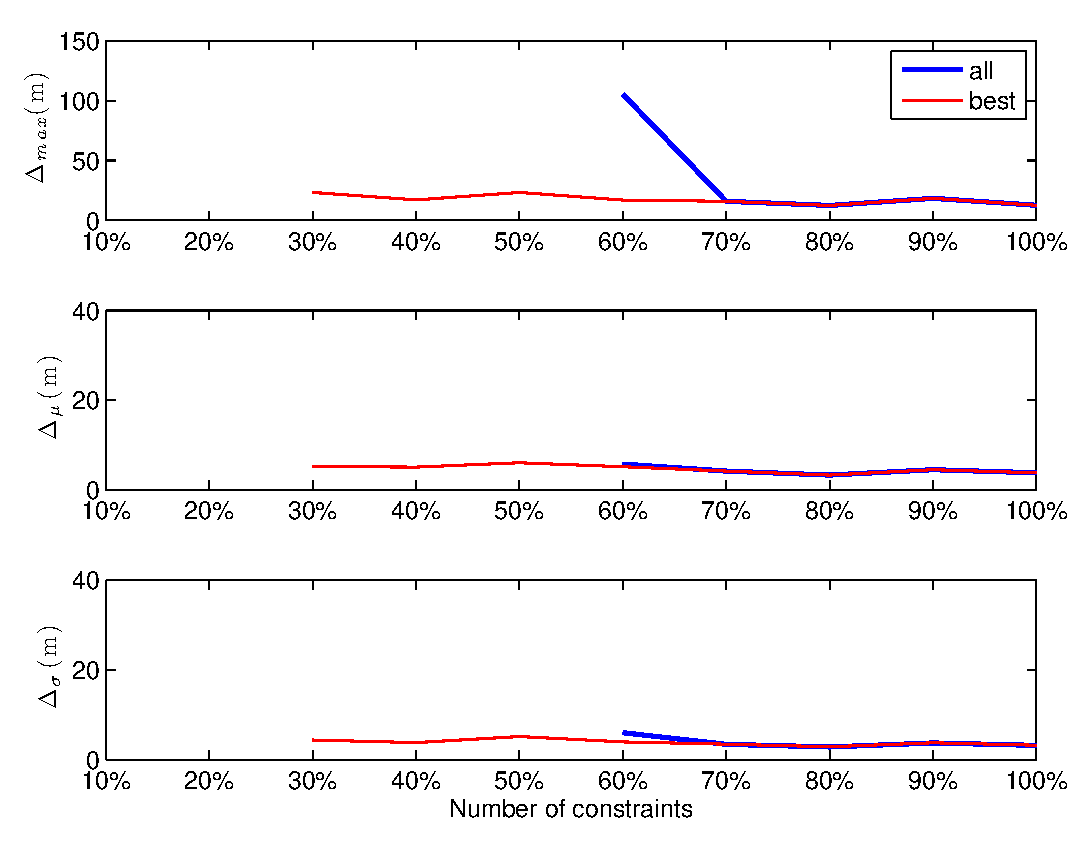
\includegraphics[width = 20pc]{../../thesis_version2/diags/eq_location_optimisation/synth3Dmulti/ressummary_3Dsynth50eq.eps}
\noindent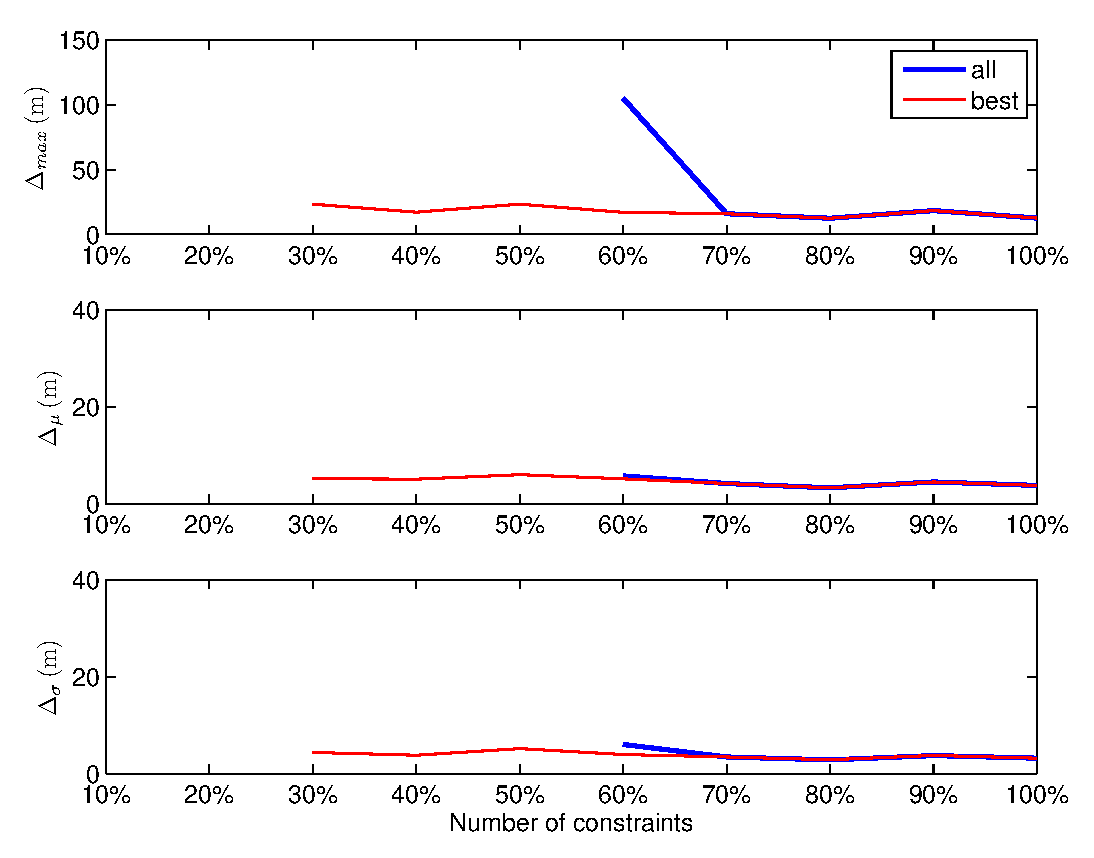
\includegraphics[width = 20pc]{diags/ressummary_3Dsynth50eq.eps}
\caption{Statistical measures of error in the optimisation solutions for the 3D synthetic cases when all (blue)
and best (red) results are considered. The statistics $\Delta_{max}$, $\Delta_\mu$ and
$\Delta_\sigma$ are the maximum, mean and standard deviation of the coordinate error, respectively.
The absence of the blue and red lines below 60\% and 30\% indicates a breakdown in the solutions
when all or best optimisation result(s) are considered, respectively.}
\label{fig:optimisationresults-3Dsynth}
\end{figure}

As in the 2D example we observe a consistency of the optimisation procedure when the number of direct links used
is high. That is, when 70\% of the direct constraints are considered all optimisation results (grey) are consistent with
the best solution (black). Furthermore, the best solution appears to constrain the event locations down to 30\%
of the direct links. There is however, one notable difference between the 3D and 2D results.
In 2D the final iteration was typically close to the actual solution
when the optimisation chain failed to converge after 1200 iterations. Contrastingly,
in 3D the optimisation appears to converge to the correct solution or fail completely, leading to a set locations which
in no way resemble the actual solution. This is depicted in Fig. \ref{fig:optimisationresults-3Dsynth}
by the absence of the grey and black lines below 60\% and 30\% of the constraints, respectively.
The reason for this difference may be due to the increased number of degrees
of freedom in 3D requiring a greater number of iterations to converge. Nevertheless, the accurate convergence of the best
solution for cases with 30\% or more of the links is encouraging for the potential
of coda wave optimisation to constrain earthquake location more generally.

\subsubsection{Summary of findings}

In summary, the synthetic examples demonstrate the ability of coda wave data to constrain event location
using optimisation. The optimisation error is influenced by the
noise on CWI estimates with greater $\bar{\sigma}_N$ leading to larger
errors in the solutions. When 70\% or more of the direct branches are used the
optimiser is stable with no observable difference in the solution for 25 randomly chosen starting
locations. As the direct linkage reduces to 50\% the optimisation becomes less stable and the best solution
from 25 random starting locations is required to find the optimal solution. Finally, as the number of links decrease
below 30\% the best solution also fails to converge to a useful result.


\section{Relocating Earthquakes on the Calaveras Fault}
\label{sec:CalaverasLoc-CWIonly}

In this section we consider real
earthquakes and undertake a complete coda wave analysis beginning with waveform selection, filtering, pairwise application
of CWI and optimisation.
\begin{itemize}
\item Introduce the Calaveras Fault and provide a brief background of why it is chosen here (Figure \ref{fig:-eqopti-California-Calaveras})
\item Discuss Catalogue Locations - hypoDD locations and CWI locations
(Figure \ref{fig-69Calaverasevents_eg1})
\begin{itemize}
\item mention difference between hypoDD inversions when 68 or
308 earthquakes considered but don't show figure (i.e. difference in coordinates for
the two solutions is roughly 2\,m)
\item provide details on CWI application - waveform selection, filtering etc.
\end{itemize}
\item Discuss comparison between CWI and catalogue locations - first order performance of CWI and clustering
\item Discuss comparison between CWI and hypoDD locations - second order result and streaks.
\end{itemize}

\begin{figure}
\noindent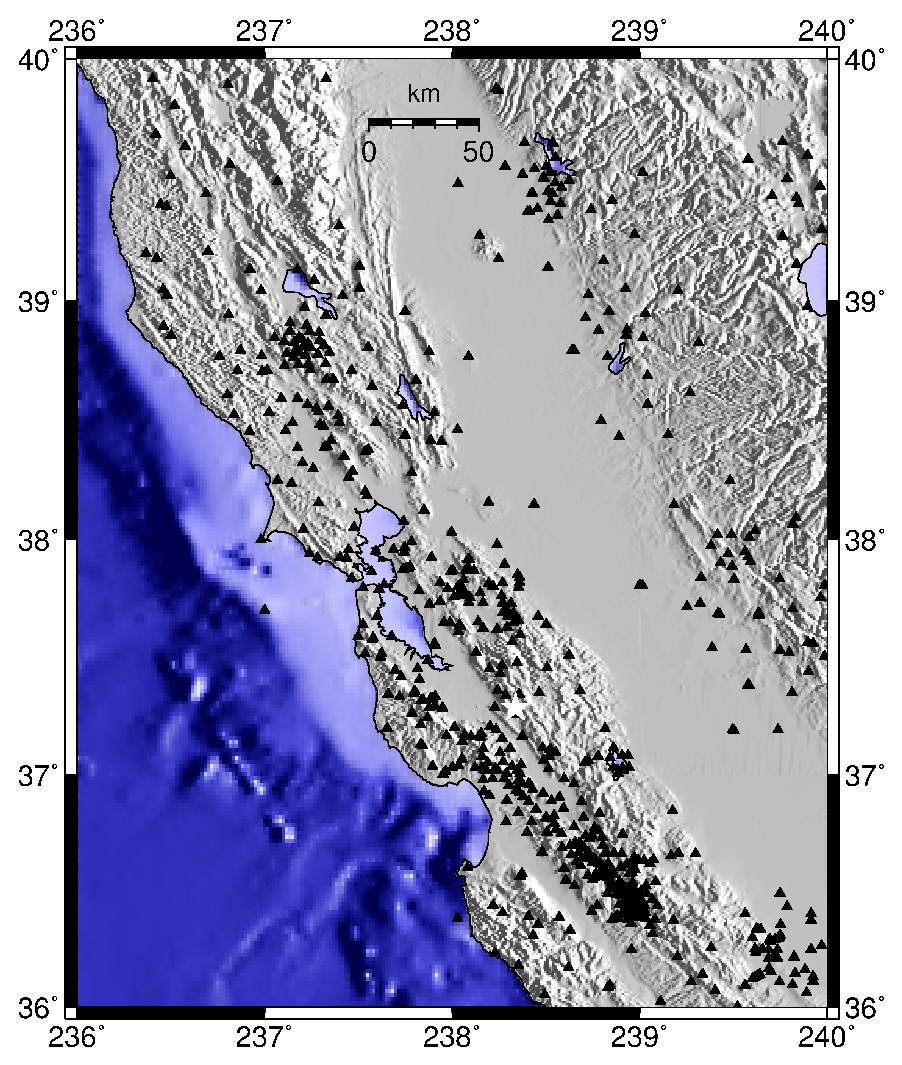
\includegraphics[width = 20pc]{diags/CalaverasMap/gmt_california/CaliforniaCalaverasMap1.eps}
\caption{Elevation in California showing location
of the 308 event Calaveras cluster (black star) and 805 seismic stations (red triangles).}
\label{fig:-eqopti-California-Calaveras}
\end{figure}


%%=======================================================================================
% This is the original figure using HypoDD with LSQR
%\begin{figure*}
%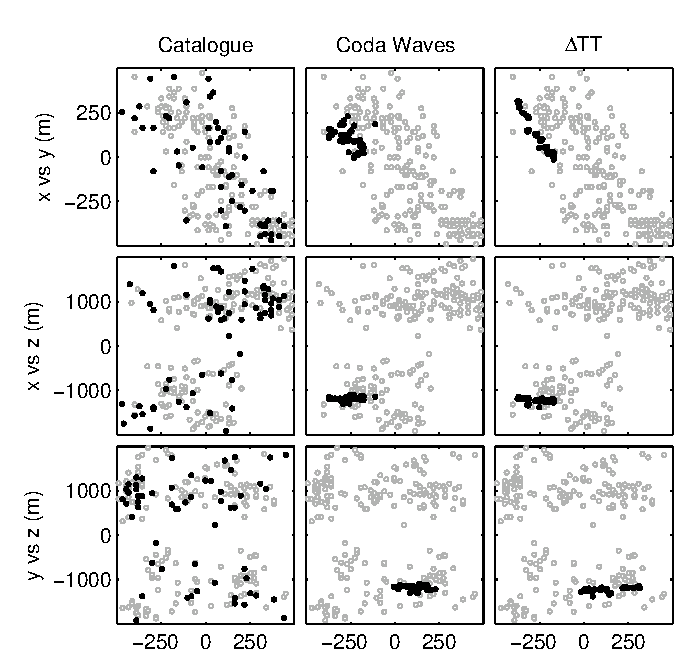
\includegraphics{diags/CalaverasLoc1.eps}
%\caption{Comparison of earthquake hypocenters using three different methods: catalogue location (column 1), hypoDD with all
%308 events (column 2) and CWI example 1 (column 3).
%Note that in the case of the CWI locations we consider only the 68 earthquakes in red, the
%blue events are shown for the purpose of orientation only.}
%\label{fig-69Calaverasevents_eg1}
%\end{figure*}

% Now we have the SVD version 
\begin{figure*}
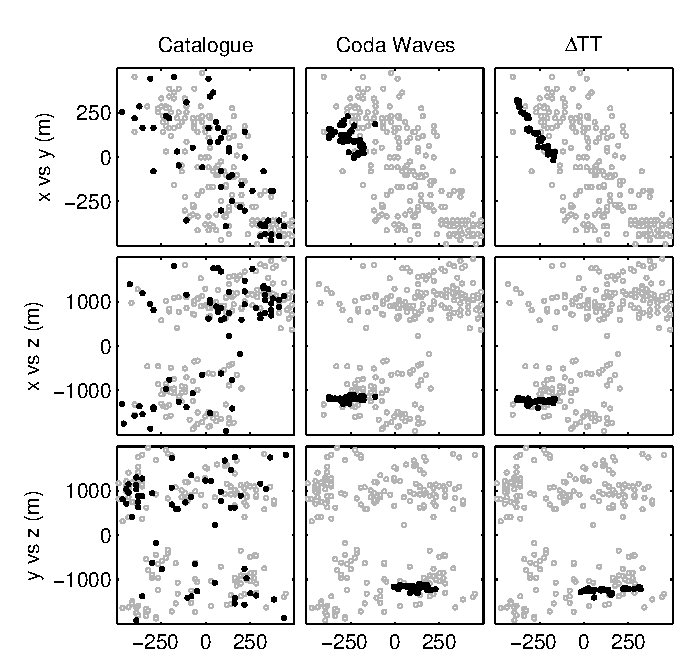
\includegraphics{diags/CalaverasLoc1_hypoDD_SVD.eps}
\caption{Comparison of earthquake hypocenters using three different methods: catalogue location (column 1), hypoDD with all
308 events (column 2) and CWI example 1 (column 3).
Note that in the case of the CWI locations we consider only the 68 earthquakes in red, the
blue events are shown for the purpose of orientation only.}
\label{fig-69Calaverasevents_eg1}
\end{figure*}
%%=======================================================================================



\subsection{Dependance on the number of stations}

\begin{itemize}
\item Explain issues associated with poor station coverage - superimpose
the three SWSZ (i.e. Australian) stations onto  Figure
\ref{fig:-eqopti-California-Calaveras}
\item Show setup for consideration of fewer stations (Table
\ref{tab:Calaveras-stationremoval}
and Figure \ref{fig:-eqopti-Calaveras-substations})
\item Show the results (Figures \ref{fig-68Calaveras_CWIxyloc-statremove}
to \ref{fig-68Calaveras_hypoDDyzloc-statremove} and Figure \ref{fig-statremoval_summarystats})
\item Discuss the better performance of CWI with fewer stations
\item Question/Discuss why hypoDD continues to suggest streaks with 2 or 3 stations - there must be regularization
\end{itemize}

\begin{figure}
\noindent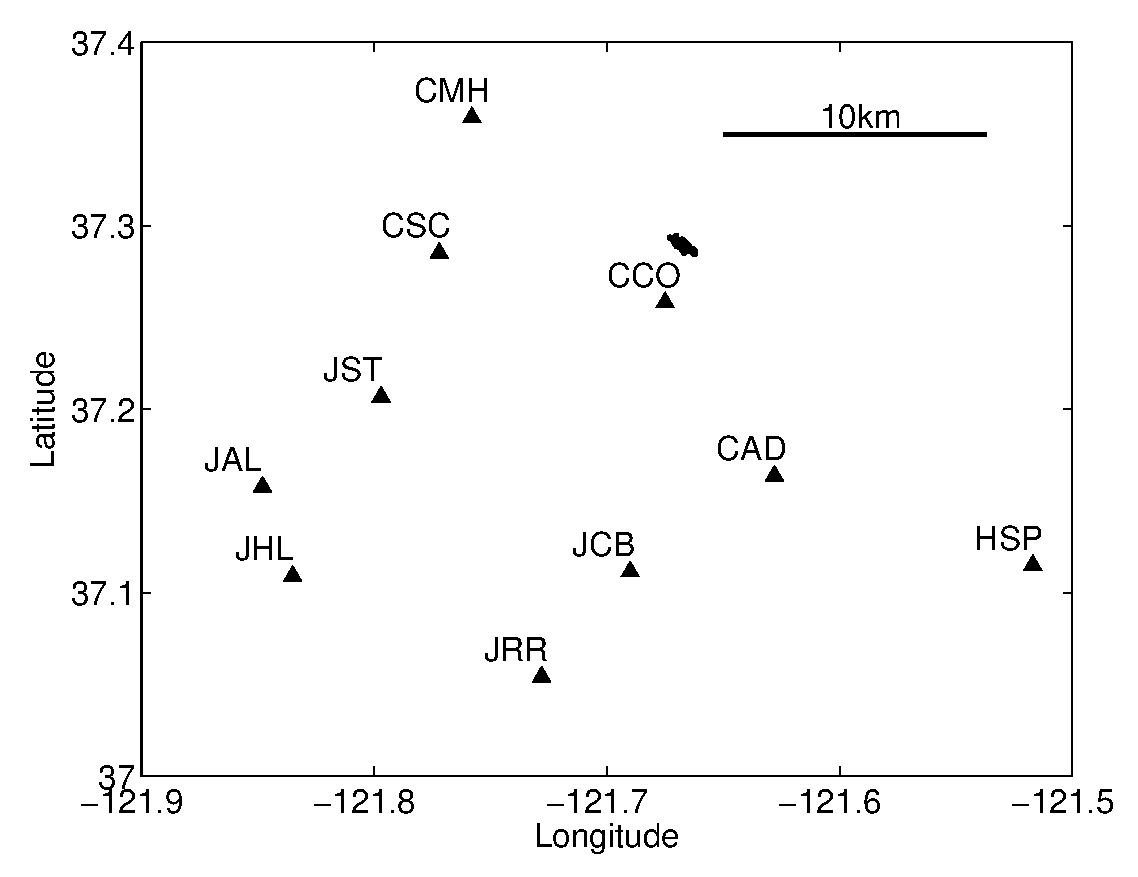
\includegraphics[width = 20pc]{diags/CalaverasMap/matlab/Calaveras_substationmap}
\caption{Location of the 10 stations (red triangles) used to relocate the Calaveras events.
Stations are removed one at a time according to the order in Table \ref{tab:Calaveras-stationremoval} and the events
relocated (see Figures \ref{fig-68Calaveras_CWIxyloc-statremove} to \ref{fig-68Calaveras_hypoDDyzloc-statremove}).
The 304 Calaveras events are indicated with black circles.}
\label{fig:-eqopti-Calaveras-substations}
\end{figure}

\begin{table}
\caption{Stations considered when exploring the effect of reduced station coverage.}
\label{tab:Calaveras-stationremoval}
\begin{tabular}{|r|l|}
\hline
Number of & Station Names\\
Stations  & \\
\hline
10 & CCO, JCB, JST, CMH, HSP, JAL, CSC, JST, CAD, JHL, JRR\\
9  & CCO, JCB, JST, CMH, HSP, JAL, CSC, JST, CAD, JHL\\
8  & CCO, JCB, JST, CMH, HSP, JAL, CSC, JST, CAD\\
7  & CCO, JCB, JST, CMH, HSP, JAL, CSC \\
6  & CCO, JCB, JST, CMH, HSP, JAL \\
5  & CCO, JCB, JST, CMH, HSP \\
4  & CCO, JCB, JST, CMH \\
3  & CCO, JCB, JST \\
2  & CCO, JCB \\
1  & CCO \\
\hline
\end{tabular}
\end{table}

\begin{figure*}
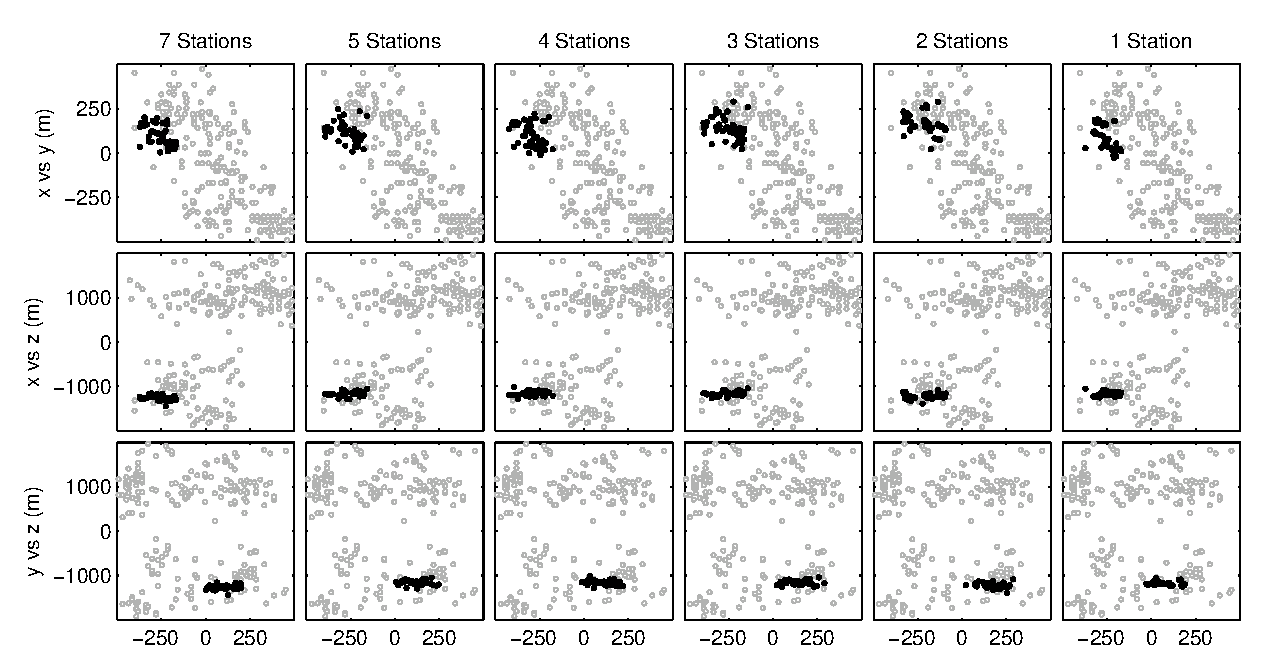
\includegraphics[angle=90,height = 50pc]{diags/CalaverasLoc2.eps}
\caption{....}
\label{fig-CWIreducesstats}
\end{figure*}


%%=========================================================================
% this is the original version using hypoDD with LSQ
%\begin{figure*}
%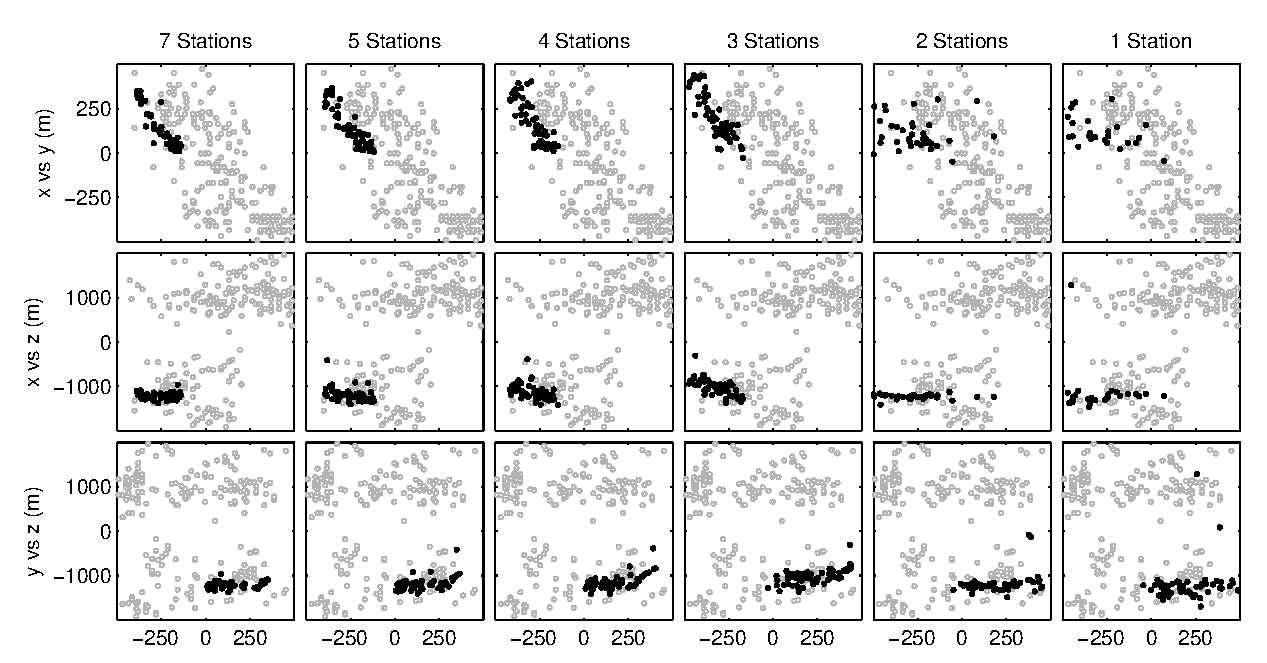
\includegraphics[angle=90,height = 50pc]{diags/CalaverasLoc3.eps}
%\caption{....}
%\label{fig-HYPODDreducesstats}
%\end{figure*}

% This is the version using hypoDD with SVD
\begin{figure*}
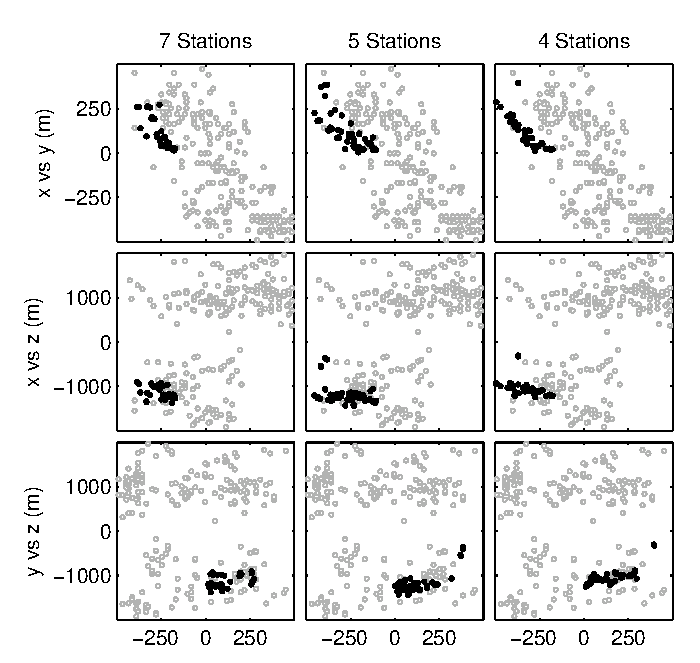
\includegraphics[height = 25pc]{diags/CalaverasLoc3_hypoDD_SVD.eps}
\caption{HypoDD (SVD) with reduced stations.}
\label{fig-HYPODDreducesstats}
\end{figure*}
%%=========================================================================


%%=========================================================================
% This is the original version using hypoDD with LSQ
%\begin{figure}
%\noindent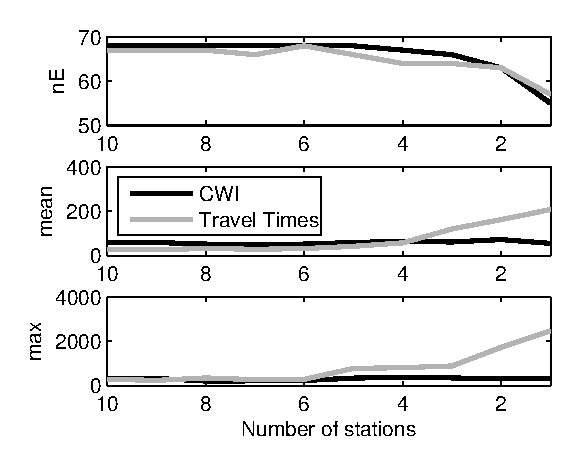
\includegraphics[width = 20pc]{diags/CalaverasLoc4.eps}
%\caption{Statistics on coordinate differences for reduced station inversions. Differences
%are computed between the inversion results (CWI and hypoDD) and the complete hypoDD
%locations for all 308 events. The top subplot illustrates the number of constrainable
%events in the CWI and hypoDD inversions as a function of the stations considered.}
%\label{fig-statremoval_summarystats}
%\end{figure}

% This is the version using hypoDD with SVD
\begin{figure}
\noindent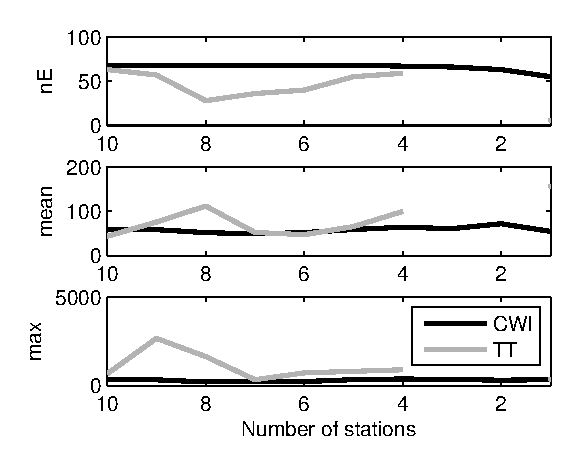
\includegraphics[width = 20pc]{diags/CalaverasLoc4_hypoDD_SVD.eps}
\caption{Statistics on coordinate differences for reduced station inversions. Differences
are computed between the inversion results (CWI and hypoDD) and the complete hypoDD
locations for all 308 events. The top subplot illustrates the number of constrainable
events in the CWI and hypoDD inversions as a function of the stations considered.}
\label{fig-statremoval_summarystats}
\end{figure}
%%=========================================================================

\section{Combining travel time and CWI constraints}
\label{sec:CalaverasLoc-CWIandTT}
\begin{itemize}
\item Pose the problem
\item Introduce the idea of a travel time based separation PDF with mean event locations from hypoDD outputs and
some measure of uncertainty (we will consider three levels of uncertainty as in paper1).
\item Explain how to combine the CWI based posterior with these new travel time based separation PDFs
\item Show the derivatives of the travel time based separation PDF
\item Undertake the combined inversion show/discuss findings (Figure \ref{fig-68Calaverasevents_ttandcoda1} )
\end{itemize}

%%=========================================================================
% This is the original version using hypoDD with LSQ
% This is only makes sense for LSQR so we remove it from this manuscript
%\begin{figure*}
%\noindent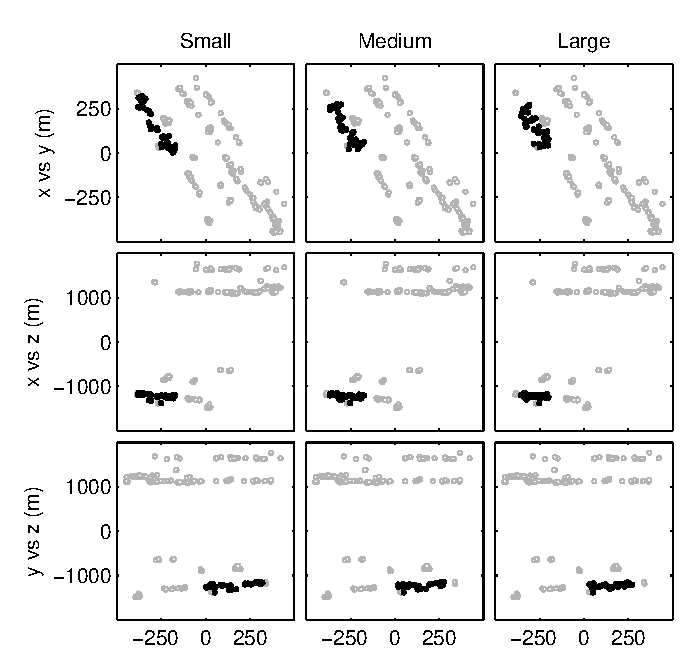
\includegraphics{diags/CalaverasLoc5.eps}
%\caption{Locations of the 68 Calaveras earthquakes combining all available coda wave and travel time constraints with three different
%levels of uncertainty on the travel time PDFs. Column 1 sets $\sigma_x = \sigma_y = 19.5$\,m and $\sigma_z = 15$\,m
%\citep[after]{dr_Waldhauser08a}, Column 2 uses $\sigma_x = \sigma_y = 3 \times19.5$\,m and $\sigma_z = 3\times15$\,m and
%column 3 considers $\sigma_x = \sigma_y = 152$\,m and $\sigma_z = 232$\,m \citep[after]{dr_Shearer97a}. }
%\label{fig-68Calaverasevents_ttandcoda1}
%\end{figure*}
%%=========================================================================


\subsection{Combining CWI and travel times when the travel times constrain a limited number of events}

\begin{itemize}
\item Explain the idea of a temporary deployment of stations i.e. for aftershocks
\item Discuss Omori formula and the $M_s$7.8 Hokkaido-Nansei-Oki earthquake
\citep[Figure \ref{fig:Omorifigure},]{dr_Utsu95a}
\item Show/Discuss results (Figure \ref{fig-68Calaverasevents_ttsubsetandcoda1})
\end{itemize}

\begin{figure}
\noindent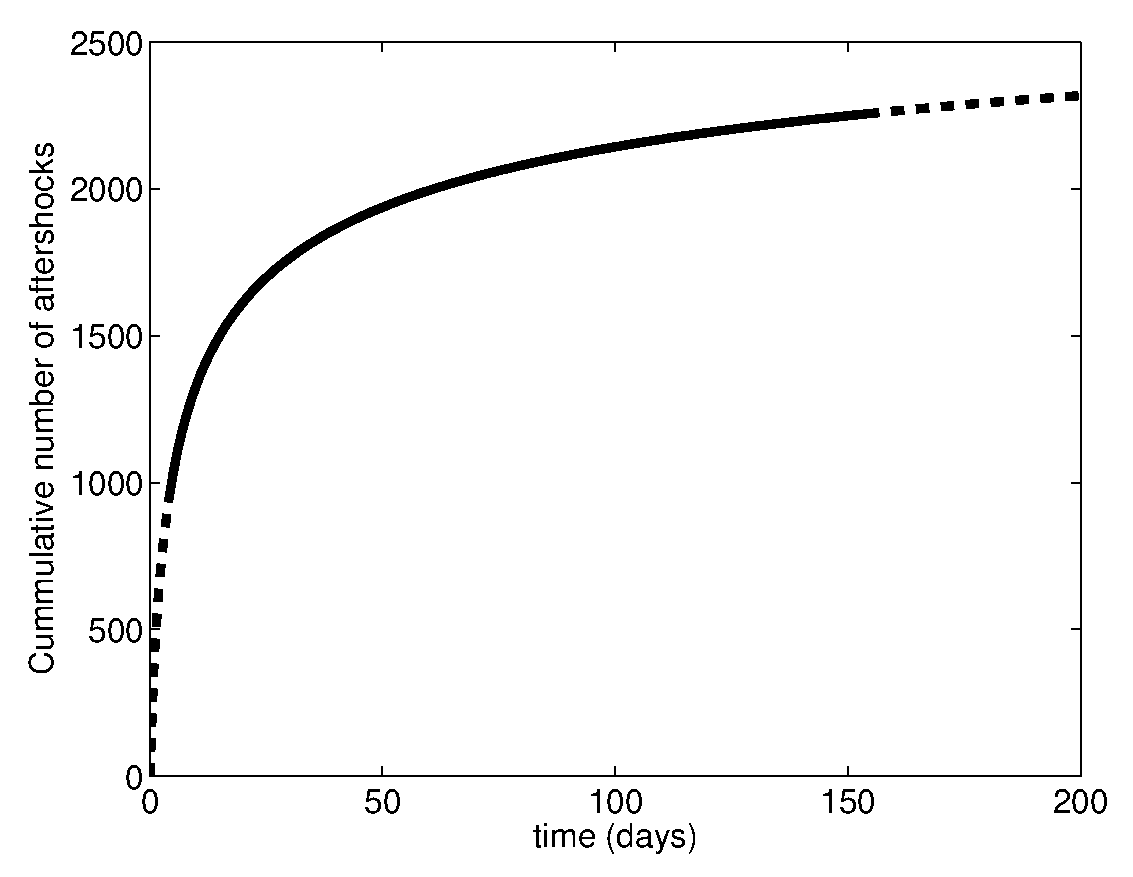
\includegraphics[width = 20pc]{diags/OmoriFigure.eps}
\caption{Cumulative number of aftershocks for the Hokkaido-Nansei-Oki, Japan
$M_s=7.8$ earthquake of 12 July 1993 according to the best fitting modified Omori Formula
\citep{dr_Utsu95a}. The leftmost dashed, middle solid and rightmost dashed signify aftershocks occurring before, during and
after the deployment of a temporary array installed 7 days after the main shock and left for
65 days.}
\label{fig:Omorifigure}
\end{figure}


%%=========================================================================
% This is the original version using hypoDD with LSQ
%\begin{figure}
%\noindent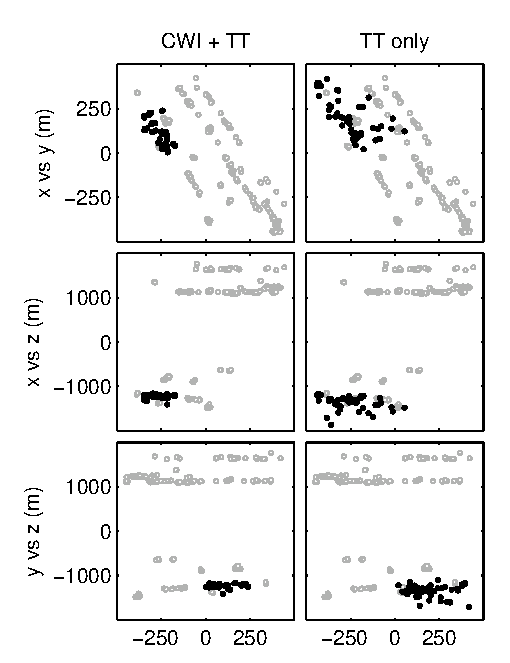
\includegraphics{diags/CalaverasLoc6.eps}
%\caption{Left - Combined travel time and coda wave inversions using travel time constraints on
%22 (or 32\%) of the events and coda waves from station CCO only. All travel time based uncertainties
%are assigned $\sigma_x = \sigma_y = 3 \times19.5$\,m and $\sigma_z = 3\times15$\,m. Right - travel time
%relocation only (i.e. no CWI) using ........}
%\label{fig-68Calaverasevents_ttsubsetandcoda1}
%\end{figure}

% This is the version using hypoDD with SVD
\begin{figure*}
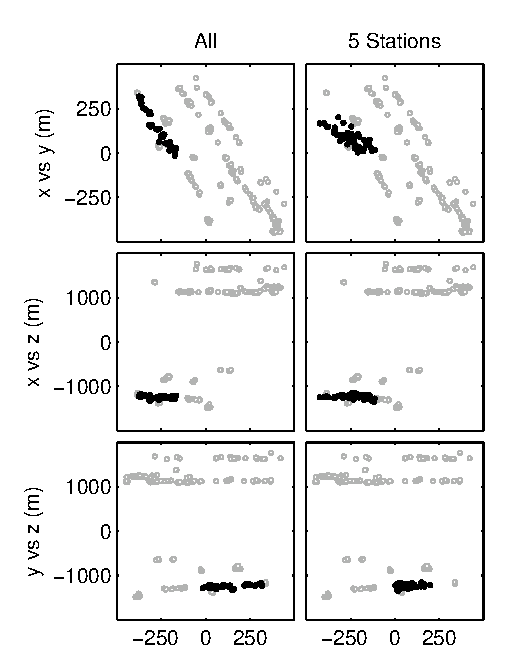
\includegraphics{diags/CalaverasLoc5_hypoDD_SVD.eps}
\caption{Combined HypoDD (SVD) and CWI: all stations and 5 stations.}
\label{fig-69Calaverasevents_eg1}
\end{figure*}
%%=========================================================================

\section{Conclusions}
\begin{itemize}
\item Emphasise strengths of the CWI relocation (i.e. with small number of stations,
linking temporary deployments with catalogue locations)
\item Discuss potential applications e.g. intraplate/downhole/tunnel monitoring etc.
\end{itemize}




\begin{acknowledgments}
(Text here)
\end{acknowledgments}


\bibliography{../../refs/drrefs}




\appendix

\section{The noisy likelihood}
\label{sec-Appendix-noisylikelihood}

The noisy likelihood $P(\widetilde{\delta}_{CWIN}|\widetilde{\delta}_t)$
used in eq. (\ref{eq:-bayesian-noisyform}) is given by
\begin{equation}
\begin{array}{l}
\label{eq-likelihood-int}
P(\widetilde{\delta}_{CWIN}|\widetilde{\delta}_t)  =
A(\widetilde{\delta}_t) C(\bar{\mu}_N, \bar{\sigma}_N)  \\
\hspace{3em} \times \int_0^\infty
B(\widetilde{\delta}_t,\widetilde{\delta}_{CWI})
D(\widetilde{\delta}_{CWI},\bar{\sigma}_N,\bar{\mu}_N )
d\widetilde{\delta}_{CWI}
\end{array}
\end{equation}
where $\widetilde{\delta}_{CWI}$ is an estimate of CWI separation in the absence
of noise,
\begin{equation}
\label{eq:Adefn}
A(\widetilde{\delta}_t) = \frac{1}{(1-\Phi_{\mu_1,\sigma_1}(0))\sigma_1\sqrt{2\pi} },
\end{equation}
\begin{equation}
B(\widetilde{\delta}_t,\widetilde{\delta}_{CWI})=e^{  \frac{-(\widetilde{\delta}_{CWI}-\mu_1)^2}{2\sigma_1^2} },
\end{equation}
\begin{equation}
\label{eq:Cdefn}
C(\bar{\mu}_N, \bar{\sigma}_N) =  \frac{1}{(1-\Phi_{\bar{\mu}_N,\bar{\sigma}_N}(0))\sigma_N\sqrt{2\pi}},
\end{equation}
\begin{equation}
D(\widetilde{\delta}_{CWI},\bar{\sigma}_N,\bar{\mu}_N )=e^{  \frac{-(\widetilde{\delta}_{CWI}-\bar{\mu}_N)^2}{2 \bar{\sigma}_N ^2} }
\end{equation}
and $\Phi_{\mu,\sigma}(x)$ is the cumulative Gaussian distribution function
\begin{equation}
\label{eq-cummulative-Gaussian}
\Phi_{\mu,\sigma}(x) = \frac{1}{\sigma \sqrt{2 \pi}}
\int_{-\infty}^x e^{  \frac{-(s-\mu)^2}{2\sigma^2}  } ds
\end{equation}
\citep{dr_Robinson10b}. The parameters $\mu_1$ and $\sigma_1$ used in
eq. (\ref{eq:Adefn}) are defined by the expresions
\begin{equation}
\label{eq:mu1}
\mu_1(\widetilde{\delta}_t) = a_1\frac{a_2 \widetilde{\delta}_t^{a_4}+a_3
\widetilde{\delta}_t^{a_5}}{a_2 \widetilde{\delta}_t^{a_4}+a_3 \widetilde{\delta_t}^{a_5}+1}
\end{equation}
and
\begin{equation}
\label{eq:sigma1}
\sigma_1(\widetilde{\delta}_t) = c + a_1\frac{a_2 \widetilde{\delta}_t^{a_4}+
a_3 \widetilde{\delta}_t^{a_5}}{a_2 \widetilde{\delta}_t^{a_4}+a_3 \widetilde{\delta}_t^{a_5}+1}
\end{equation}
with coefficients $a_1$ to $a_5$ and $c$ defined in Table \ref{tab-const4-mu1-sigma1}.
The parameters $\bar{\mu}_N$ and $\bar{\sigma}_N$ used in
eq. (\ref{eq:Cdefn}) are obtained by finding the values which minimise the
difference in a least squares sense between the noisy CWI estimates $\widetilde{\delta}_{CWIN}$
computed from the waveforms and the
positively bounded Gaussian density function
\begin{equation}
\label{eq-likelihood-noisydata-pdf-orig}
\begin{array}{l}
P(\widetilde{\delta}_{CWIN}|\widetilde{\delta}_t,\widetilde{\delta}_{CWI}) \\
\hspace{5em} = \frac{1}{\left(1-\Phi_{\bar{\mu}_N,\bar{\sigma}_N}(0)\right)\bar{\sigma}_N\sqrt{2\pi}}
e^{  \frac{-(\widetilde{\delta}_{CWIN}-\bar{\mu}_N)^2}{2\bar{\sigma}_N^2}  }
\end{array}
\end{equation}
with $\widetilde{\delta}_{CWIN} \geq 0$.


\begin{table}
\caption{Coefficients for eqs. (\ref{eq:mu1}) and (\ref{eq:sigma1}).}
\label{tab-const4-mu1-sigma1}
\begin{tabular}{|c|c|}
\hline
$\mu_1(\widetilde{\delta}_t)$ & $\sigma_1(\widetilde{\delta}_t)$ \\
\hline
$a1 = 0.4661$ & $a1 = 0.1441$\\
$a2 = 48.9697$ & $a2 = 101.0376$\\
$a3 = 2.4693$ & $a3 = 120.3864$\\
$a4 = 4.2467$ & $a4 = 2.8430$\\
$a5 = 1.1619$ & $a5 = 6.0823$ \\
     & $c = 0.017$ \\
\hline
\end{tabular}
\end{table}


\section{Derivatives}
\label{sec-Appendix-derivatives_ofL}

The derivatives of $L(\mathbf{e}_1,\mathbf{e}_2,...,\mathbf{e}_N)$
\begin{equation}
\frac{\partial L}{\partial \hat{x}_1},
\frac{\partial L}{\partial \hat{y}_1},
 \frac{\partial L}{\partial \hat{z}_1},
\frac{\partial L}{\partial \hat{x}_2},
\frac{\partial L}{\partial \hat{y}_2},
\frac{\partial L}{\partial \hat{z}_2},
...,
\frac{\partial L}{\partial \hat{x}_N},
\frac{\partial L}{\partial \hat{y}_N},
\frac{\partial L}{\partial \hat{z}_N}
\end{equation}
are required by the Polak-Ribiere algorithm. These are used to guide the optimisation procedure
towards the values of $(\mathbf{e}_1,\mathbf{e}_2,...,\mathbf{e}_N)$ which
minimise $L$.

The equations for the derivatives are convoluted so we
build them gradually. We start with an expression for $\delta_t$, the wavelength normalised separation between two events
$\mathbf{e}_p= (\hat{x}_p,\hat{y}_p,\hat{z}_p)$ and $\mathbf{e}_q = (\hat{x}_q,\hat{y}_q,\hat{z}_q)$
\begin{equation}
\label{eq:deltat4chapt6deriv}
\delta_t = \frac{f_{dom}}{v_s}\sqrt{(\hat{x}_p-\hat{x}_q)^2 + (\hat{y}_p-\hat{y}_q)^2 +  (\hat{z}_p-\hat{z}_q)^2},
\end{equation}
where $f_{dom}$ is the dominant frequency of the waveforms and $v_s$ is the velocity between the events. Expression
\ref{eq:deltat4chapt6deriv} has derivatives
\begin{equation}
\label{eq-partial-xyz1}
\begin{array}{l}
\frac{\partial \widetilde{\delta}_t}{\partial \hat{x}_p} = \frac{f_{dom}^2 (\hat{x}_p-\hat{x}_q)}{v_s^2 \widetilde{\delta}_t},
\frac{\partial \widetilde{\delta}_t}{\partial \hat{y}_p} = \frac{f_{dom}^2 (\hat{y}_p-\hat{y}_q)}{v_s^2 \widetilde{\delta}_t}, \\
\frac{\partial \widetilde{\delta}_t}{\partial \hat{z}_p} = \frac{f_{dom}^2 (\hat{z}_p-\hat{z}_q)}{v_s^2 \widetilde{\delta}_t},
\frac{\partial \widetilde{\delta}_t}{\partial \hat{x}_q} = \frac{f_{dom}^2 (\hat{x}_q-\hat{x}_p)}{v_s^2 \widetilde{\delta}_t}, \\
\frac{\partial \widetilde{\delta}_t}{\partial \hat{y}_q} = \frac{f_{dom}^2 (\hat{y}_q-\hat{y}_p)}{v_s^2 \widetilde{\delta}_t},
\frac{\partial \widetilde{\delta}_t}{\partial \hat{z}_q} = \frac{f_{dom}^2 (\hat{z}_q-\hat{z}_p)}{v_s^2 \widetilde{\delta}_t}.
\end{array}
\end{equation}
For brevity we focus the following derivation in terms of $\hat{x}_p$. The remaining terms for $\mathbf{e}_p$
(i.e. $\hat{y}_p$ and $\hat{z}_p$) can be computed
by following the same procedure. The derivatives for $\mathbf{e}_q$ can be attained by exploiting the symmetry
\begin{equation}
\label{eq:ep2eq-deriv-symmetry}
\frac{\partial \widetilde{\delta}_t}{\partial \hat{x}_q} = - \frac{\partial \widetilde{\delta}_t}{\partial \hat{x}_p}.
\end{equation}

The chain rule gives
\begin{equation}
\frac{\partial \mu_1}{\partial \hat{x}_p} = \frac{\partial \mu_1}{\partial \widetilde{\delta}_t} \frac{\partial \widetilde{\delta}_t}{\partial \hat{x}_p}
\end{equation}
where differentiating eq. (\ref{eq:mu1}) gives
\begin{equation}
\label{eq-dmu1-by-dx1}
\frac{\partial \mu_1}{\partial \widetilde{\delta}_t} = a_1 \frac{a_2 a_4 \widetilde{\delta}_t^{a_4-1} +a_3 a_5 \widetilde{\delta}_t^{a_5-1}}
{\left(a_2 \widetilde{\delta}_t^{a_4} +a_3 \widetilde{\delta}_t^{a_5} +1 \right)^2}.
\end{equation}
Similarly, we have
\begin{equation}
\frac{\partial \sigma_1}{\partial \hat{x}_p} = \frac{\partial \sigma_1}{\partial \widetilde{\delta}_t} \frac{\partial \widetilde{\delta}_t}
{\partial \hat{x}_p}
\end{equation}
where $\frac{\partial \sigma_1}{\partial \widetilde{\delta}_t}$ has the identical form as \ref{eq-dmu1-by-dx1} with different constants
$a_1,a_2,...,a_5$ (see table \ref{tab-const4-mu1-sigma1}).

The cumulative Gaussian distribution function \ref{eq-cummulative-Gaussian} is
\begin{equation}
\Phi_{\mu_1,\sigma_1}(0) = \frac{1}{\sigma_1 \sqrt{2 \pi}}
\int_{-\infty}^0 e^{  \frac{-(s-\mu_1)^2}{2\sigma_1^2}  } ds
\end{equation}
which has derivative
\begin{equation}
\frac{\partial \Phi_{\mu_1,\sigma_1}(0)}{\partial \hat{x}_p} =
\frac{ \sigma_1 \int_{-\infty}^0 \frac{\partial g}{\partial \hat{x}_p} e^g ds -
\frac{\partial \sigma_1}{\partial \hat{x}_p} \int_{-\infty}^0 e^g ds}
{\sigma_1^2 \sqrt{2 \pi}}
\end{equation}
where
\begin{equation}
g = \frac{-(s-\mu_1)^2}{2 \sigma_1^2}
\end{equation}
and
\begin{equation}
\frac{\partial g}{\partial \hat{x}_p} = \frac{4 \sigma_1^2 (s-\mu_1) \frac{\partial \mu_1}{\partial \hat{x}_p}
+ 4\sigma_1 \frac{\partial \sigma_1}{\partial \hat{x}_p}(s-\mu_1)^2}
{4 \sigma_1^4}.
\end{equation}

Now, we have all the pieces to compute the derivatives of $A=A(\delta_t)$ and $B = B(\delta_t,\delta_{CWI})$ as follows
\begin{equation}
\frac{\partial A} {\partial \hat{x}_p} =
-\frac{ -\frac{\partial  \Phi_{\mu_1,\sigma_1}(0)}{\partial \hat{x}_p} \sigma_1 +
 \left(1- \Phi_{\mu_1,\sigma_1}(0) \right) \frac{\partial \sigma_1}{\partial \hat{x}_p}}
{\left(1- \Phi_{\mu_1,\sigma_1}(0) \right)^2 \sigma_1^2 \sqrt{2 \pi}}
\end{equation}
and
\begin{equation}
\frac{\partial B} {\partial \hat{x}_p} = e^h \frac{\partial h}{\partial \hat{x}_p}
\end{equation}
where
\begin{equation}
h =  \frac{-(\delta_{CWI}-\mu_1)^2}{2 \sigma_1^2}
\end{equation}
and
\begin{equation}
\frac{\partial h}{\partial \hat{x}_p} = \frac{
4 \sigma_1^2 (\delta_{CWI}-\mu_1) \frac{\partial \mu_1}{\partial \hat{x}_p}
+ 4(\delta_{CWI}-\mu_1)^2 \sigma_1 \frac{\partial \sigma_1}{\partial \hat{x}_p} }
{4 \sigma_1^4}.
\end{equation}
Finally, we can differentiate the likelihood for an individual event pair
\begin{equation}
\begin{array}{l}
\frac{\partial P(\delta_{CWIN}|\widetilde{\delta}_t)} {\partial \hat{x}_p}  =
\frac{\partial A(\widetilde{\delta}_t)}{\partial \hat{x}_p} C(\bar{\mu}_N, \bar{\sigma}_N) \\
\hspace{2em} \times \int_0^\infty B(\widetilde{\delta}_t,\widetilde{\delta}_{CWI})
D(\widetilde{\delta}_{CWI},\bar{\sigma}_N,\bar{\mu}_N )
d\widetilde{\delta}_{CWI} \\
\hspace{2em} + A(\widetilde{\delta}_t) C(\bar{\mu}_N, \bar{\sigma}_N) \\
\hspace{2em} \times \int_0^\infty
\frac{\partial B(\widetilde{\delta}_t,\widetilde{\delta}_{CWI})} {\partial \hat{x}_p}
D(\widetilde{\delta}_{CWI},\bar{\sigma}_N,\bar{\mu}_N )
d\widetilde{\delta}_{CWI}
\end{array}
\end{equation}
and for the logarithm we have
\begin{equation}
\frac{ \partial \ln \left[ P(\delta_{CWIN}|\delta_t) \right] } {\partial \hat{x}_p}
= \frac{1}{P(\delta_{CWIN}|\delta_t)} \frac{\partial P(\delta_{CWIN}|\delta_t)}{\partial \hat{x}_p}.
\end{equation}


Thus, it follows that the derivative of $L$ with respect to $\hat{x}_p$ is given by
%\begin{equation}
%\label{eq-derivative-Lstar-cwionly22}
%\frac{\partial L(E_1, E_2, ..., E_n)}{\partial \hat{x}_p} =
%- \sum_{i=p+1}^{N} \frac{ \partial \ln \left[P(\delta_{CWIN}|E_p,E_i)\right]}{\partial \hat{x}_p}
%+ \sum_{j=1}^{p-1} \frac{ \partial \ln \left[P(\delta_{CWIN}|E_j,E_p)\right]}{\partial \hat{x}_p}
%\end{equation}
\begin{equation}
\label{eq-derivative-Lstar-cwionly}
\begin{array}{ll}
\frac{\partial L(E_1, E_2, ..., E_n)}{\partial \hat{x}_p} = &
- \sum_{i=p+1}^{N} \frac{ \partial \ln \left[P(\delta_{CWIN}|E_p,E_i)\right]}{\partial \hat{x}_p} \\
 & + \sum_{j=1}^{p-1} \frac{ \partial \ln \left[P(\delta_{CWIN}|E_j,E_p)\right]}{\partial \hat{x}_p}
\end{array}
\end{equation}
%
%\iftwocol{\begin{eqnarray} \frac{\partial L(E_1, E_2, ..., E_n)}{\partial \hat{x}_p} &  = &\\
%- \sum_{i=p+1}^{N} \frac{ \partial \ln \left[P(\delta_{CWIN}|E_p,E_i)\right]}{\partial \hat{x}_p} \\
%+ \sum_{j=1}^{p-1} \frac{ \partial \ln \left[P(\delta_{CWIN}|E_j,E_p)\right]}{\partial \hat{x}_p}
%\end{eqnarray}}
%{\frac{\partial L(E_1, E_2, ..., E_n)}{\partial \hat{x}_p} =
%- \sum_{i=p+1}^{N} \frac{ \partial \ln \left[P(\delta_{CWIN}|E_p,E_i)\right]}{\partial \hat{x}_p}
%+ \sum_{j=1}^{p-1} \frac{ \partial \ln \left[P(\delta_{CWIN}|E_j,E_p)\right]}{\partial \hat{x}_p}}
%\end{equation}
for a uniform prior. The change of sign in the middle (i.e. to addition) accounts for the change in
order of the events under the conditional. Its inclusion here assumes the correct use of
$\partial \widetilde{\delta}_t / \partial \hat{x}_p$
or
$\partial \widetilde{\delta}_t / \partial \hat{x}_q$
when evaluating the left and right hand terms of the summation. The derivatives shown in this section
appear complicated but are in practice trivial to compute numerically.
Confidence in their accuracy is enhanced in the following sections by demonstrating that
the optimisation procedure converges to the correct solution for a number of synthetic problems
in 2 and 3 dimensions.


\clearpage








%\bsp % ``This paper has been produced using the Blackwell
     %   Publishing GJI \LaTeXe\ class file.''

\label{lastpage}


\end{document}
